\chapter*{\chapterstyle{VI --- Introduction}}
\addcontentsline{toc}{section}{Introduction}

Dans ce chapitre nous étudions les propriétés analytiques et de régularité d'un ensemble plus général de fonctions, les \textbf{fonctions d'un espace vectoriel normé dans un autre} et plus précisément, on se concentrera principalement sur le cas des fonctions de \(\R^n\) dans \(\R^p\).\<

Soit \(\mathcal{D}\) une partie de \(\R^n\) et \((x_1, \ldots, x_n) \in \mathcal{D}\), on considère alors la fonction:
\[
   \begin{aligned}
      f : \mathcal{D} \subseteq \R^n &\longrightarrow \R^p \\
      (x_1, \ldots, x_n) &\longmapsto (f_1(x), \ldots, f_p(x))
   \end{aligned}
\]
On dira alors que la fonction \(f_i\) est la i-ème application \textbf{composante} de \(f\).\+

\subsection*{\subsecstyle{Définitions{:}}}
On peut alors définir quelques notions de vocabulaire:
\begin{itemize}
   \item Si la fonction est à valeur scalaire, on dira que c'est \textbf{un champ de scalaires}.
   \item Si la fonction est à valeur vectorielles, on dira que c'est \textbf{un champ de vecteurs}.
\end{itemize}

\subsection*{\subsecstyle{Représentations{:}}}
On cherche alors à représenter de telles fonctions, on sait que dans le cas élémentaire des fonctions à une seule variable, on peut représenter le \textbf{graphe} d'une fonction \(f\) donné par:
\[
   \mathcal{G}_f := \bigl\{ (x, f(x)) \in \R^2 \; ; \; x \in \R \bigl\}   
\]
Dans le cas d'une fonction de plusieurs variables, on peut alors généraliser cette définition par:
\[
   \mathcal{G}_f := \bigl\{ (x, f(x)) \; ; \; x \in \R^n \bigl\}  
\]

De façon générale, le graphe d'une fonction de \(\R^n\) dans \(\R^p\) est un objet à \(n\) dimensions dans l'espace à \((n + p)\) dimensions (les points sont caractérisés par \(n\) paramètres, en termes
savants on dira qu'il s'agit d'une sous-variété de \(\R^{(n + p)}\) de dimension \(n\).\<

Si on considère par exemple une fonction de \(\R^2\) dans \(\R\), c'est alors une fonction qui à chaque point du plan associe une valeur numérique, qu'on peut alors représenter comme \textbf{une hauteur} et on obtient alors \textbf{une surface}, par exemple:

\begin{figure}
   \centering
   \vspace*{-0.5cm}
   \begin{tikzpicture}
      \begin{axis}[domain=-1.5:1.5,y domain=-1.5:1.5, scale=1, colormap={custom}{color(0)=(DarkBlue3) color(1)=(BrightBlue1)}]
        \addplot3[draw=black, opacity=0.5, surf, samples=40] {exp(-x^2-y^2)};
      \end{axis}
    \end{tikzpicture}
   \captionsetup{labelformat=empty}
   \caption{Graphe de la fonction \(f : (x, y) \mapsto \exp(-x^2 - y^2)\)}
\end{figure}
\pagebreak

Dans le cas général néanmoins, il est plus difficile de représenter ce type de fonctions mais on peut par exemple s'inspirer des fonctions \(\C \rightarrow \C\) et utiliser la \textbf{couleur} comme 4-ème dimension de l'image. On peut aussi de manière heuristique représenter simplement le domaine de départ et/ou d'arrivée pour étudier le comportement de la fonction.

\subsection*{\subsecstyle{Cas des champs de vecteurs{:}}}
De manière générale, le caractère multidimensionnel de l'espace d'arrivée importe peu dans tout le chapitre qui va suivre, les notions analytiques étant définies à partir d'une limite, elles passeront aux composantes comme les notions évoquées au chapitre précédent.\<

Dans toute la suite on considèrera alors souvent le cas épuré de champs de scalaires et il est attendu d'adapter les résultat élémentaires aux cas à valeurs vectorielles.

\subsection*{\subsecstyle{Lignes de niveaux{:}}}
On considère une fonction \(f : \R^2 \rightarrow \R\), alors on appelle \textbf{ligne de niveau} associé à la valeur \(\lambda\) l'ensemble suivant:
\[
   L_\lambda := \Bigl\{ (x, y) \in \R^2 \; ; \; f(x, y) = \lambda \Bigl\}   
\]
C'est une courbe plane qui représente l'ensemble des points du plan ou la fonction prends une valeur fixée, tracer plusieurs lignes de niveaux permet alors d'obtenir des informations sur la fonction, par exemple:
\begin{figure}[h]
   \centering
   \begin{tikzpicture}[line cap=round, scale=2]
      \tkzInit[xmin=-2,xmax=2,ymin=-2,ymax=2]
      \draw[-latex] (-2,0) -- (2,0) node [right] {$x$};
      \draw[-latex] (0, -2) -- (0,2) node [above] {$y$};
      \tkzFctPar[samples=400,domain=0:2*pi, color=BrightRed1, line width=0.3mm]{0.226480229573*cos(t)}{0.226480229573*sin(t)};       
      \tkzFctPar[samples=400,domain=0:2*pi, color=BrightRed2, line width=0.3mm]{0.536360021303*cos(t)}{0.536360021303*sin(t)}; 
      \tkzFctPar[samples=400,domain=0:2*pi, color=DarkGreen1, line width=0.3mm]{0.83255461115*cos(t)}{0.83255461115*sin(t)};      
      \tkzFctPar[samples=400,domain=0:2*pi, color=DarkGreen2, line width=0.3mm]{1.17741002252*cos(t)}{1.17741002252*sin(t)};      
      \tkzFctPar[samples=400,domain=0:2*pi, color=DarkGreen3, line width=0.3mm]{1.51742712939*cos(t)}{1.51742712939*sin(t)};
      \draw node[color=BrightRed1] at (0.27, 0.27) {\scriptsize $L_{0.95}$};
      \draw node[color=BrightRed2] at (0.49, 0.49) {\scriptsize $L_{0.75}$};
      \draw node[color=DarkGreen1] at (0.7, 0.7) {\scriptsize $L_{0.50}$};
      \draw node[color=DarkGreen2] at (0.95, 0.95) {\scriptsize $L_{0.25}$};
      \draw node[color=DarkGreen3] at (1.2, 1.2) {\scriptsize $L_{0.10}$};
   \end{tikzpicture}
   \captionsetup{labelformat=empty}
   \caption{Lignes de niveau de la fonction \(f : (x, y) \mapsto \exp(-x^2 - y^2)\)}
\end{figure}

\subsection*{\subsecstyle{Changements de variables{:}}}
L'étude des fonctions à plusieurs variables va nous amener à étudier les \textbf{changements de variables} que nous allons définir:
\begin{center}
   \textbf{On appelle changement de variable tout \(\mathcal{C}^k\) difféomorphisme entre deux espaces.}
\end{center}
En particulier, on verra que le passage en coordonées polaires défini comme suite est bien un changement de variable et en tant que tel, il préserve les propriétés différentielles:
\[
   \begin{aligned}
      \phi : \R_+^* \times \ioo{-\pi}{\pi} &\longrightarrow \R^2 \backslash (\R_- \times \{0\})\\
      (r, \theta) &\longmapsto (r\cos(\theta), r\sin(\theta))
   \end{aligned}
\]

\chapter*{\chapterstyle{VI --- Limite \& Continuité}}
\addcontentsline{toc}{section}{Limite \& Continuité} 
Dans ce chapitre nous définirons le concept de limite dans le cas d'une fonction à plusieurs variables, plus précisément, sauf exceptions, dans le cas d'un champ de scalaire. Dans les cas ou les généralités sont triviales, on utilisera sans vergogne l'exemple canonique d'une fonction \(f : \R^2 \rightarrow \R\)

\subsection*{\subsecstyle{Définition{:}}}
On considère \(f : \R^p \rightarrow \R\), alors une telle fonction admet une limite \(l\) en \(a\) si et seulement si:
\[
   \forall\, V_l \in \mathscr{V}_l \; , \; \exists\, V_a \in \mathscr{V}_a \; ; \; f(V_a) \subseteq V_l
\]
Graphiquement, cela signife simplement que peu importe le voisinage \(V\) de la limite que l'on considère,
il sera possible de trouver un voisinage de \(a\) tel que tout ses points soient envoyés dans \(V\).\<

Le caractère métrique de l'espace de départ nous permet d'avoir la caractérisation en termes de boules:
\[
   \forall \epsilon >0 \; , \; \exists \lambda > 0 \; , \; \forall x \in \R^n \; , \; \vectNorm{x - a} < \lambda \implies |f(x) - l| < \epsilon
\]
On obtient évidemment aussi toutes les autres variantes possibles (limites en \(\pm \infty\) notamment). Dans le cas d'un champ de vecteurs, on définit de manière générale:
\[
   \forall \epsilon >0 \; , \; \exists \lambda > 0 \; , \; \forall x \in \R^n \; , \; \vectNorm{x - a}_{\R^n} < \lambda \implies \vectNorm{f(x) - l}_{\R^p} < \epsilon
\]
On notera alors:
\[
   \lim_{(x, y) \rightarrow (a, b)} f(x, y) = l
\]
\subsection*{\subsecstyle{Limites suivant une restriction{:}}}
Cette définition correspond bien à l'intuition \textit{topologique} de la notion de limite. En particulier, on peut alors montrer que si \(f\) tends vers \(l\) en \((a, b)\), alors en particulier si on considère un \textbf{chemin} de la forme:
\[
   \gamma : t \mapsto (\gamma_1(t), \gamma_2(t))   
\]
Et si ce chemin est tel qu'il passe par \((a, b)\) en \(t_0\), alors on a nécessairement:
\[
   \lim_{(x, y) \rightarrow (a, b)} f(x, y) = l \implies \lim_{t \rightarrow t_0} f(\gamma(t)) = l
\]
En particulier cela nous permet de construire une méthode pour démontrer la \textbf{non-existence de limite}, ie:
\begin{center}
   \textit{Si il existe deux chemins différents suivant lesquels la fonction admets deux limites différentes, alors elle n'admet pas de limite en ce point.}
\end{center}
\subsection*{\subsecstyle{Erreurs communes{:}}}
Cette définition correspond bien à l'intuition \textit{topologique} de la notion de limite. Néanmoins il faut remarquer les propriétés suivantes spécifiques aux fonctions à plusieurs variables:
\begin{itemize}
   \item Il est possible qu'une fonction admette une limite suivant plusieurs chemins, mais pas de limite.
   \item Il est meme possible qu'une fonction admette une limite suivant toutes les droites, mais pas de limite.
   \item De manière générale, admettre une limite sur plusieurs restrictions ne permet pas d'affirmer l'existence d'une limite.
\end{itemize}

\subsection*{\subsecstyle{Opérations{:}}}
Comme dans le cas des fonctions réelles, on peut alors démontrer les propriétés opératoires de la limite, en effet si on considère \(f, g\) deux champs scalaires qui admettent deux limites \(l_1, l_2\) en \(A \in \R^p\),alors on a les propriétés suivantes:
\begin{itemize}
   \item Le passage à la limite est \textbf{linéaire}.
   \item Le passage à la limite est \textbf{multiplicatif}.
   \item Le passage à la limite (non-nulle) d'une fonction localement non-nulle est \textbf{inversible}.
\end{itemize}
La première propriété se généralise aux champs vectoriels, mais pas les deux secondes bien évidemment, car les opérations en jeu (effectuées à l'arrivée) ne sont pas définies pour des vecteurs.\<

Enfin pour deux fonction qui sont composables, on a la propriété fondamentale suivante:
\begin{itemize}
   \item Le passage à la limite est compatible avec la \textbf{composition}.
\end{itemize}

\subsection*{\subsecstyle{Caractérisation séquentielle{:}}}
Comme dans le cas des fonctions réelles on a la caractérisation séquentielle de la limite, en effet une fonction \(f\) tends vers \(l\) en \((a, b)\) si et seulement si pour tout suite \((u_n)\) qui tends vers \((a, b)\), on a:
\[
   \lim_{n \rightarrow +\infty} f(u_n) = l
\]
\begin{center}
   \textit{En particulier, si on arrive à trouver deux suites qui tendent vers \((a, b)\) telles que \(f(u_n)\) et \(f(v_n)\) tendent vers deux valeurs différentes, alors la limite de \(f\) ne peut pas exister.}
\end{center}

\subsection*{\subsecstyle{Théorème d'encadrement {:}}}
On peut généraliser le théorème des gendarmes aux fonctions à plusieurs variables, en effet si on considère \(f, g, h\) trois fonctions telles que \(f(x, y) \leq g(x, y) \leq h(x, y)\) dans un voisinage de \((a, b)\) alors on a:
\[
   \lim_{(x, y) \rightarrow (a, b)} f(x, y) = \lim_{(x, y) \rightarrow (a, b)} h(x, y) = l \implies \lim_{(x, y) \rightarrow (a, b)} g(x, y) = l
\] 
En particulier si \((a, b) = (0, 0)\), et si \(|f(x, y)| \leq g(x, y)\), alors:
\[
   \lim_{(x, y) \rightarrow (a, b)} g(x, y) = 0 \implies \lim_{(x, y) \rightarrow (a, b)} f(x, y) = 0
\]

\subsection*{\subsecstyle{Passage en polaire {:}}}
Si on considère une fonction à deux variables, on peut exprimer \((x, y)\) en coordonées polaires, ie considérer la composée \(f(x, y) = f(r\cos(\theta), r\sin(\theta))\) et alors \(f\) tends vers \(0\) en \((0, 0)\) si et seulement si il existe une fonction \(g(r)\) telle que:
\[
   |f(r\cos(\theta), r\sin(\theta))| \leq g(r)
\]
Avec \(g(r)\) qui tends vers \(0\) quand \(r\) tends vers \(0\). \textbf{Attention} la fonction \(g\) ne doit plus dépendre de \(\theta\).

\chapter*{\chapterstyle{VI --- Continuité}}
\addcontentsline{toc}{section}{Continuité}   
De manière similaire au cas réel, on dira alors qu'une fonction est \textbf{continue} en un point \(A\) si et seulement si:
\[
   \lim_{(x, y) \rightarrow (a, b)} f(x, y) = f(a, b)   
\]
Et toute les propriétés opératoires usuelles sont alors aisément démontrées. En particulier, on peut montrer que toutes les fractions rationnelles sont continues sur leur ensemble de définition, et donc tout les polynomes.

\subsection*{\subsecstyle{Applications linéaires {:}}}
Soit \(f : E \rightarrow F\) une application linéaire, alors on a le théorème fondamental suivant qui énonce que \(f\) est continue sur son domaine de définition si et seulement si elle vérifie une des conditions équivalentes suivantes:
\begin{itemize}
   \item Elle est continue en 0.
   \item Elle est bornée sur la boule unité.
   \item Sa \textbf{norme d'opérateur} est bornée.
\end{itemize}
Et on définit la norme d'opérateur d'une application linéaire par:
\[
   |||f||| = \underset{x \in E \backslash \{0_E\}}{\sup}{\frac{||u(x)||}{||x||}}   
\]
En particulier, muni des ces équivalences, on peut démontrer la propriétés fondamentale suivante:
\begin{center}
   \textbf{En dimension finie, toutes les applications linéaires sont continues.}
\end{center}

\subsection*{\subsecstyle{Caractére local {:}}}
Le fait d'admettre une limite ou d'etre continue est une propriété dite \textbf{locale}, cela signifie que pour que la propriété soit vraie, il faut que des propriétés soit vérifiées dans \textbf{un voisinage} d'un point. En particulier, on peut remarquer des propriétés importantes:
\begin{center}
   Si \(f = g\) sur un \textbf{ouvert} \(U\), et que \(f\) est vérifie une propriété \textbf{locale} sur \(A\), alors \(g\) la vérifie aussi.
\end{center}
Cette propriété est en générale \textbf{fausse} sur une partie qui n'est pas ouverte.

\chapter*{\chapterstyle{VI --- Dérivées Directionnelles}}
\addcontentsline{toc}{section}{Dérivées Directionnelles} 
Dans ce chapitre nous essaierons de construire un concept de \textbf{dérivée} dans le cas d'une fonction à plusieurs variables, plus précisément, sauf exceptions, dans le cas d'un champ de scalaire. Dans les cas ou les généralités sont triviales, on utilisera sans vergogne l'exemple canonique d'une fonction \(f : \R^2 \rightarrow \R\)

\subsection*{\subsecstyle{Applications Partielles {:}}}
On considère une fonction de \(A \subseteq \R^p \rightarrow \R\) et un point \(a = (a_1, \ldots, a_n)\) \textbf{intérieur} à \(A\). Alors il existe un voisinage de \(a\) ou la fonction \textbf{réelle} suivante est bien définie, on l'appelle alors \textbf{i-ème application partielle} au point \(a\):
\[
   \begin{aligned}
      f_{x_i} : \R &\longrightarrow \R\\
      t &\longmapsto f(a_1, \ldots, t, \ldots, a_n)
   \end{aligned}
\]
\begin{center}
   \textit{Considèrer la i-ème application partielle, c'est fixer une direction et considèrer la courbe de \(f\) suivant cette direction.}
\end{center}
Géométriquement, on peut le voir comme l'interesection d'un plan parallèle à l'axe considéré et passant par \(a\), et l'application partielle est alors l'intersection de la courbe et du plan:
\begin{figure}[h]
   \centering
   \begin{tikzpicture}
      \begin{axis}[domain=-1.5:1.5,y domain=-1.5:1.5, scale=1, colormap={custom}{color(0)=(DarkBlue3) color(1)=(BrightBlue1)}]
         \addplot3[draw=black, opacity=0.5, surf, samples=40] {exp(-x^2-y^2)};
         \addplot3[draw=DarkBlueX, line width = 0.5mm, samples=51, samples y=0,domain=-1.5:1.5,variable=\t]
         ({\t},{-0.5},{exp(-\t^2 - 0.5^2)});         
      \end{axis}
    \end{tikzpicture}
   \captionsetup{labelformat=empty}
   \caption{Application partielle \(f_x\) en \((0, -0.5)\) de \(f : (x, y) \mapsto \exp(-x^2 - y^2)\)}
\end{figure}
\subsection*{\subsecstyle{Dérivées Partielles {:}}}
On dira alors qu'une telle fonction \textbf{admet une i-ème dérivée partielle} au point \(a\) si et seulement si sa i-ème application partielle en \(a\) est dérivable en \(a_i\). On se ramène alors à l'étude de la dérivabilité d'une fonction \textbf{réelle}, ce qui ne pose pas de problème théorique. Dans ce cas, on notera alors:
\[
   \frac{\partial f}{\partial x_i}(a) = f_{x_i}'(a_i)   
\]
Si \(f\) admet une i-ème dérivée partielle sur un ouvert \(\mathcal{U}\) si et seulement si elle en admet en tout points de \(\mathcal{U}\) et on définit alors:
\[
   \begin{aligned}
      \frac{\partial f}{\partial x_i} : \mathcal{U} &\longrightarrow \R\\
      a &\longmapsto \frac{\partial f}{\partial x_i}(a_i)
   \end{aligned}
\]
On dira alors qu'un fonction à plusieurs variables est de classe \(\mathcal{C}^k\) en un point si elle admet toutes ses dérivées partielles en ce point et qu'elles y sont continues.
\pagebreak
\subsection*{\subsecstyle{Propriétés opératoires{:}}}
On peut montrer que la dérivation partielle est un \textbf{opérateur différentiel} agissant sur un espace de fonctions qui admettent des dérivées partielles, en particulier en utilisant les définitions précédentes et en notant \(\mathcal{D}_i(\R^n)\) l'espace des fonctions admettant une i-ème dérivée partielle, alors on peut définir:
\[
   \begin{aligned}
      \frac{\partial}{\partial x_i} : \mathcal{D}_i(\R^n) &\longrightarrow \mathcal{F}(\mathcal{U}, \R)\\
      f &\longmapsto \frac{\partial f}{\partial x_i}
   \end{aligned}
\]

C'est donc cet opérateur que nous appliquons à une fonction qui admet des dérivées partielles. En particulier, l'intéret de cette définition est alors de pouvoir affirmer les propriétés suivantes:
\begin{itemize}
   \item La dérivation partielle est \textbf{linéaire}.
   \item La dérivation partielle suit \textbf{la règle du produit}.
\end{itemize}
La première propriété se généralise aux champs vectoriels, mais pas la seconde bien évidemment, car les opérations en jeu (effectuées à l'arrivée) ne sont pas définies pour des vecteurs.\<

\underline{Exemple:} On considère les fonctions suivantes en un point \((x, y)\):
\[
   \begin{aligned}
      f : (x, y) &\longmapsto xy \quad\quad\quad g : (x, y) &\longmapsto x^2y
   \end{aligned}
\]
Alors on a\footnote[1]{\textbf{Attention:} Ici on fait l'abus de notation usuel d'utiliser deux fois la variable \(x\) qui ont deux sens différents, l'expression \(\partialD{fg}{x}\) signifie simplement qu'on dérive par rapport à la première variable (penser \(\partial_1(fg)\)) et \((x, y)\) représente le point d'évaluation de la dérivée partielle.)}:
\[
   \partialD{(fg)}{x}(x, y) = \partialD{f}{x}(x, y)g(x, y) + \partialD{g}{x}(x, y)f(x, y) = yx^2y + 2xyxy = 3x^2y^2
\]
On voit bien ici que la dérivée d'un produit n'a de sens que si on est dans le cas de (au moins un) champs scalaires !
\subsection*{\subsecstyle{Dérivée partielle d'une composée{:}}}
Le cas de la composée est plus subtil et on reviens temporairement au cas général des deux champs vectoriels suivants dont on supposera qu'ils admettent toutes leurs dérivées partielles partout:
\[
   \begin{aligned}
      g : \R^m &\longmapsto \R^n \quad\quad\quad f : \R^n &\longmapsto \R^p
   \end{aligned}
\]
On cherche à caculer la dérivée partielle par rapport à la \(i\)-ème variable de la fonction \(f \circ g\) au point \(a\), on peut alors montrer la formule suivante, appellée \textbf{chain rule}: 
\[
   \partialD{(f \circ g)}{x_i}(a) = \sum_{k=1}^{n} \partialD{g_k}{x_i}(a)\partialD{f}{x_k}(g(a))
\]
\underline{Exemple:} On considère un fonction \(f : \R^2 \rightarrow \R\) de classe \(\mathcal{C}^1\) et la fonction \(g\) de passage en polaire:
\[
   \begin{aligned}
      g : (r, \theta) &\longmapsto (r\cos(\theta), r\sin(\theta))
   \end{aligned}
\]
On se propose de calculer la première dérivée partielle de \(f \circ g\) au point \((r, \theta)\), on a alors:
\begin{flalign*}
   \partialD{(f \circ g)}{r}(r, \theta) 
   &= \partialD{g_1}{r}(r, \theta)\partialD{f}{x}(r\cos(\theta), r\sin(\theta)) + \partialD{g_2}{r}(r, \theta)\partialD{f}{y}(r\cos(\theta), r\sin(\theta))\\ 
   &= cos(\theta)\partialD{f}{x}(r\cos(\theta), r\sin(\theta)) + sin(\theta)\partialD{f}{y}(r\cos(\theta), r\sin(\theta))
\end{flalign*}
\subsection*{\subsecstyle{Dérivées partielles d'ordre supérieur {:}}}
La i-ème dérivée partielle de \(f\) étant à nouveau une fonction de \(n\) variables, on peut alors considèrer ses dérivées partielles. On définit les dérivées partielles secondes de \(f\) (si elles existent), notées:
\[
   \frac{\partial^2 f}{\partial x_i \partial x_j}(a)   
\]
Et par récurrence les dérivées partielles d'ordre \(k\) par:
\[
   \frac{\partial^k f}{\partial x_{i_1} \ldots \partial x_{i_k}}(a)
\]
Et on se pose alors la question de l'importance de \textbf{l'ordre de dérivation} et de manière générale, on peut alors montrer que l'ordre d'application de l'opérateur compte, ie que:
\[
   \frac{\partial^2 f}{\partial x_j \partial x_i}(a) \neq \frac{\partial^2 f}{\partial x_i \partial x_j}(a)
\]
Mais le théorème de Schwarz donne alors une condition suffisante pour que l'ordre ne compte pas:
\begin{center}
   \textbf{Si les dérivées partielles sont toutes continues en un point, alors l'ordre de dérivation n'importe pas.}
\end{center}
\subsection*{\subsecstyle{Dérivées Directionnelles A REVOIR {:}}}
On peut alors généraliser cette définition en considèrant une direction quelconque, dirigée par un vecteur \(v\), et on dira alors que \(f\) admet une \textbf{dérivée directionelle} au point \(a\) suivant le vecteur \(v\) si et seulement si l'application suivante est dérivable en \(0\):
\[
   \phi_v : t \mapsto f(a + tv) Uniformiser
\]
Dans ce cas, on notera alors:
\[
   \partial_v f(a) = \phi_v'(a)   Uniformiser
\]
On peut alors remarquer que les dérivées partielles ne sont alors qu'un cas particulier de dérivée directionnelle pour \(v = e_k\) Uniformiser
\subsection*{\subsecstyle{Inconvénients de cette définition{:}}}
On aimerait alors que cette définition remplisse les memes roles que ceux remplis par la dérivée usuelle, mais ce n'est pas du tout le cas, en particulier, on a les problèmes suivants:
\begin{itemize}
   \item Un fonction qui admet des dérivées partielles en un point peut ne pas etre continue en ce point.
   \item Un fonction qui admet toute ses dérivées directionnelles en un point peut ne pas etre continue en ce point.
   \item Elles ne permettent pas directement de définir une application affine tangente à la courbe.
   \item Elles ne permettent pas d'étudier les extrema de la fonction.
\end{itemize}
\begin{center}
   \textit{En résumé, le concept de dérivée directionnelle manque de puissance.}
\end{center}

\chapter*{\chapterstyle{VI --- Différentielle}}
\addcontentsline{toc}{section}{Différentielle} 
Nous allons à présent définir le vrai concept équivalent à la dérivée usuelle, qui nous permettra de généraliser l'idée d'application tangente en un point, d'étudier les extrema d'une fonction et d'étudier toutes les propriétés différentielles d'une fonction à plusieurs variables de manière générale.\<

Dans toute la suite, on s'appropriera la notation suivante des vecteurs de la \textbf{base duale}\footnote[1]{Formellement, il s'agit d'un \textbf{champ de formes 1-linéaire} (on dira aussi \textbf{1-forme différentielle}) qui à chaque point \(a\) de \(\R^n\) associe la projection canonique sur la i-ème coordonée de "l'espace tangent" en \(a\), mais dans ce cas, \(T\R^n = \R^n\), donc le champ de forme linéaire se réduit simplement en une simple forme linéaire (ou plutot un champ constant).} de \(\R^n\):
\[
   \begin{aligned}
      dx_i : (x_1, \ldots, x_n) &\longmapsto x_i 
   \end{aligned}
\]
\subsection*{\subsecstyle{Cas réel{:}}}
On rappelle qu'on dit qu'une fonction réelle \(f\) est dérivable en \(a\) de nombre dérivé \(f'(a)\) si et seulement si\footnote[2]{Ce qui est équivalent à dire que \(f(a + h) - f(a) - f'(a)h = o(|h|)\) au voisinage de \(0\)}:
\[
   \forall h \in \R \; ; \; \frac{f(a + h) - f(a) - f'(a)h}{h} \underset{h \rightarrow 0}{\longrightarrow} 0
\]
Cette definition revient alors à dire que l'application linéaire qui approxime le mieux \(f\) en \(a\) est donnée par:
\[
   \begin{aligned}
      df_a : \R &\longrightarrow \R\\
      x &\longmapsto f'(a)dx(x) = f'(a)x 
   \end{aligned}  
\]
Ce qui correspond à dire que la fonction \(df_a(x) = f'(a)x\) est \textbf{l'application linéaire tangente} à \(f\) au point \(a\). Attention, ici on dit bien linéaire, et donc ce n'est pas une tangente géométrique à la courbe, mais son pendant affine l'est.\<

On définit alors la \textbf{différentielle} de \(f\) comme la fonction qui a tout point ou \(f\) est dérivable, lui associe son application linéaire tangente, ie:
\[
   \begin{aligned}
      df : \R &\longrightarrow \mathcal{L(\R, \R)}\\
      a &\longmapsto f'(a)dx
   \end{aligned}  
\]
\begin{center}
   \textit{C'est cette notion de différentiabilité et d'application linéaire tangente qui va se généraliser dans tout sa force au cas général.}
\end{center}
\subsection*{\subsecstyle{Définition{:}}}
Soit \(f : \R^n \rightarrow \R^p\), on dira que \(f\) est \textbf{différentiable} en un point \(a\) si et seulement si il existe une application linéaire \(df_a : \R^n \rightarrow \R^p\) telle que:
\[
   \forall h \in \R^n \; ; \; \frac{f(a + h) - f(a) - df_a(h)}{\vectNorm{h}} \underset{h \rightarrow 0}{\longrightarrow} 0
\]
Ou en d'autre termes qu'il existe \(\epsilon_a\) une fonction définie sur un voisinage de \(0\), telle que \(\epsilon_a(h) \underset{h \rightarrow 0}{\rightarrow} 0\) et que: 
\[
   \forall h \in \R^n \; ; \; f(a + h) - f(a) - df_a(h) = \vectNorm{h}\epsilon_a(h)
\]
En outre, si \(f\) est différentiable sur un ouvert \(U\), alors on définit sa différentielle de la meme manière que dans le cas réel par:
\[
   \begin{aligned}
      df : \R^n &\longrightarrow \mathcal{L}(\R^n, \R^p)\\
      a &\longmapsto df_a
   \end{aligned}  
\]
Mais cette définition ne nous permet pas de connaitre la \textbf{forme} de la différentielle, et donc de la calculer, on doit donc chercher des conditions nécessaires sur cette fonction dans la section suivante. 

\subsection*{\subsecstyle{Forme nécessaire de la différentielle{:}}}
En exprimant les applications partielles de \(f\) et en utilisant la définition de la différentielle appliqué au quotient obtenu, on montre tout d'abord que \(f\) admet nécessairement toutes ses dérivées partielles en \(a\) et on a:
\[
   \partialD{f}{x_i}(a) = df_a(e_i)   
\]
Alors, en exprimant un vecteur \(x \in \R^n\) dans la base canonique et en utilisant la linéarité de la différentielle, on obtient l'expression:
\[
   df_a(x) = \sum_{k=1}^{n}x_i df_a(e_i) = \sum_{k=1}^{n} \partialD{f}{x_i}(a) x_i = \sum_{k=1}^{n} \partialD{f}{x_i}(a) dx_i
\]
Finalement, on a bien donné une forme nécessaire à la différentielle de \(f\) et on a:
\[
   \begin{aligned}
      df : \R^n &\longrightarrow \mathcal{L}(\R^n, \R^p)\\
      a &\longmapsto \sum_{k=1}^{n} \partialD{f}{x_i}(a) dx_i
   \end{aligned}  
\]
C'est bien une application linéaire à valeurs dans \(\R^p\) car par composantes \(\partialD{f}{x_i}(a)\) est un vecteur et le produit \(vdx\) est bien défini car \(dx\) est une forme linéaire.\<

\underline{Exemple:} On considère la fonction \(f : (x, y) \mapsto (xy, x + y)\), dont on souhaite calculer la différentielle en \(a = (1, 1)\) alors on a:
\[
   \begin{cases}
      \partialD{f}{x}(x, y) = (y, 1)\\
      \partialD{f}{y}(x, y) = (x, 1)
   \end{cases}   
\]
Donc la différentielle est donnée par:
\[
   df : (a, b) \mapsto (b, 1)dx + (a, 1)dy
\]
Et donc la différentielle en \(a\) est donnée par:
\[
   df_a : (x, y) \mapsto (1, 1)x + (1, 1)y = (x + y, x + y)
\]

\subsection*{\subsecstyle{Propriétés opératoires{:}}}
Tout d'abord, on peut montrer que \textbf{l'opérateur de différentiation} sur les applications différentiables sur un ouvert \(\mathcal{U}\), qu'on notera \(\mathscr{D}_a\), est un opérateur différentiel:
\[
   \begin{aligned}
      d : \mathscr{D}_\mathcal{U} &\longrightarrow \mathcal{F}(\mathcal{U}, \mathcal{L}(\R^n, \R^p))\\
      f &\longmapsto df
   \end{aligned}
\]
C'est donc cet opérateur que nous appliquons à une fonction qui admet une différentielle. En particulier, l'intéret de cette définition est alors de pouvoir affirmer les propriétés suivantes:
\begin{itemize}
   \item La différentiation est \textbf{linéaire}.
   \item La différentiation suit \textbf{la règle du produit}.
\end{itemize}
La première propriété se généralise aux champs vectoriels, mais pas la seconde bien évidemment, car les opérations en jeu (effectuées à l'arrivée) ne sont pas définies pour des vecteurs.

\subsection*{\subsecstyle{Différentielle d'une composée{:}}}
On a aussi pour \(f : \R^n \rightarrow \R^m\) différentiable en \(a\) et \(g : \R^m \rightarrow \R^p\) différentiable en \(f(a)\) la formule de différentielle d'une composée:
\[
   d(g \circ f)_a = dg_{f(a)} \circ df_a   
\]
Une autre interpretation de cette propriété sera possible plus tard via l'introduction de la Jacobienne.

\subsection*{\subsecstyle{Différentielle d'une réciproque{:}}}
Si on a \(f : \R^n \rightarrow \R^m\) un \textbf{homéomorphisme} différentiable en \(a\) et si \(df_a\) est bijective alors \(f^{-1}\) est différentiable en \(f(a)\) et on a:
\[
   d(f^{-1})_{f(a)} = (d(f)_a)^{-1}   
\]
Une autre interpretation de cette propriété sera possible plus tard via l'introduction de la Jacobienne.

\subsection*{\subsecstyle{Propriétés de régularité{:}}}
Nous nous devons maintenant de confirmer que cette définition est bien celle qui étends l'idée de dérivabilité classique. Et en effet c'est le cas et on a les propriétés suivantes:
\begin{center}
   \textbf{Si une application est différentiable, elle est continue.}
\end{center}
La réciproque est bien évidemment fausse.
\subsection*{\subsecstyle{Condition nécessaire de différentiabilité{:}}}
On aimerait maintenant réussir à trouver une condition nécessaire de différentiabilité, en effet, étudier la limite donnée par la définition est pénible et souvent complexe.\+
On montre alors la propriété fondamentale suivante:
\begin{center}
   \textbf{Si une application est de classe \(\mathcal{C}^1\), alors elle est différentiable.}
\end{center}
Ce qui nous permet simplement de calculer les dérivées partielles de \(f\) et d'étudier leur continuité pour en déduire la différentiabilité (dans les cas simples). Attention, ce n'est qu'une condition \textbf{suffisante}.
\subsection*{\subsecstyle{Plan Tangent{:}}}
Si on revient à des problématiques plus pratiques, et notamment dans le cas d'une fonction \(f : \R^2 \rightarrow \R\), alors on sait que la différentielle est l'application linéaire tangente au point \(a\), et on aimerait avoir une expression de l'application \textbf{affine} tangente en \((a, b)\), et de manière analogue au cas réel, on peut définir:
\[
   \tau_{(a, b)} := \Bigl\{ (x, y, z) \in \R^3 \; ; \; z = df_a(x - a, y - b) + f(a, b) \Bigl\}    
\]
C'est le \textbf{plan affine tangent} à la courbe de \(f\) au point \((a, b)\).

\begin{figure}[h]
   \centering
   \begin{tikzpicture}
      \begin{axis}[domain=-1.5:1.5,y domain=-1.5:1.5, scale=1, colormap={custom}{color(0)=(DarkBlue3) color(1)=(BrightBlue1)}]
        \addplot3[draw=black, opacity=0.5, surf, samples=40] {exp(-x^2-y^2)};
      \end{axis}
    \end{tikzpicture}
   \captionsetup{labelformat=empty}
   \caption{Graphe de la fonction \(f : (x, y) \mapsto \exp(-x^2 - y^2)\)}
\end{figure}
On définit de meme \textbf{l'espace affine tangent} à la courbe de \(f\) au point \((a_1, \ldots, a_n)\) par:
\[
   \tau_{(a_1, \ldots, a_n)} := \Bigl\{ (x_1, \ldots, x_n, z) \in \R^{n+1} \; ; \; z = df_a(x_1 - a_1, \ldots, x_n - a_n) + f(a_1, \ldots, a_n) \Bigl\}    
\]

\subsection*{\subsecstyle{Gradient{:}}}
On va maintenant définir un autre opérateur différentiel sur l'ensemble des fonctions de classe \(\mathcal{C}^1(\R^n, \R)\), attention, ici il s'agit bien du cas particulier des champs de scalaires. On définit alors \textbf{l'opérateur gradient}:
\[
   \begin{aligned}
      \nabla : \mathcal{C}^1(\R^n, \R) &\longrightarrow \mathcal{L}(\R^n, \R^n)\\
      f &\longmapsto \nabla f = \left(\partialD{f}{x_1}, \ldots, \partialD{f}{x_n}\right)
   \end{aligned}
\]
Le gradient de \(f\) est donc un \textbf{champ de vecteurs}, dont on verra une interprétation ci-dessous, mais tout d'abord, on peut remarquer l'identité suivante en un point \(a\), qui le lie avec la différentielle:
\[
   \forall h \in \R^n \; ; \; \dotproduct{\nabla f(a)}{h} = \dotproduct{\left(\partialD{f}{x_1}, \ldots, \partialD{f}{x_n}\right)}{h} = df_a(h)
\]

On cherche maintenant à interpréter ce que représente le gradient par rapport au champs scalaire \(f\), et on peut alors montrer la propriété géométrique suivante:
\begin{center}
   \textit{Le gradient est le champ de vecteurs qui donne la direction de la plus grand pente ascendante à la surface de la courbe de \(f\).}
\end{center}
\begin{figure}[h]
   \centering
   \vspace*{-0.5mm}
   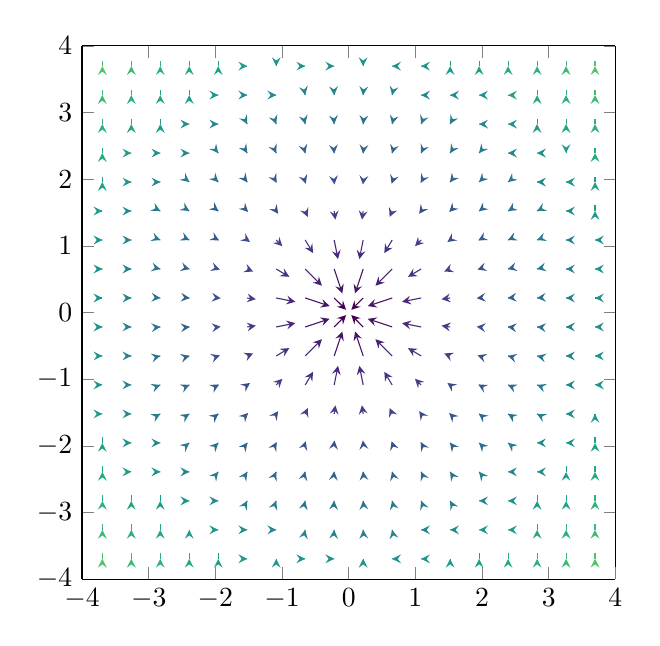
\begin{tikzpicture}
      \begin{axis}[%
         xmin = -4, xmax = 4,
         ymin = -4, ymax = 4,
         zmin = 0, zmax = 1,
         axis equal image,
         xtick distance = 1,
         ytick distance = 1,
         view = {0}{90},
         scale = 1.25,
         height=7cm,
         colormap/viridis,
      ]
      \addplot3[point meta = {sqrt(x^2+y^2)}, quiver={u=-2*x*exp(-x^2-y^2), v=-2*y*exp(-x^2-y^2), scale arrows=0.45}, quiver/colored = {mapped color}, samples=24, -stealth] (x,y,0);
     \end{axis}
   \end{tikzpicture}
   \captionsetup{labelformat=empty}
   \caption{Gradient de la fonction \(f : (x, y) \mapsto \exp(-x^2 - y^2)\)}
\end{figure}
Une autre propriété remarquable du gradient est qu'il est toujours \textbf{orthogonal} aux lignes de niveaux.

\subsection*{\subsecstyle{Jacobienne{:}}}
On considère maintenant plus généralement l'espace des fonctions de classe \(\mathcal{C}^1(\R^n, \R^p)\), et on définit alors l'opérateur suivant:
\[
   \begin{aligned}
      J : \mathcal{C}^1(\R^n, \R^p) &\longrightarrow \mathcal{M}_{p, n}(\mathcal{F}(\R^n, \R^p))\\
      f &\longmapsto \begin{pmatrix}
         \partialD{f_1}{x_1} &\ldots &\partialD{f_1}{x_n}\\
         \vdots &\ddots &\vdots \\ 
         \partialD{f_p}{x_1} &\ldots &\partialD{f_p}{x_n}
      \end{pmatrix}
   \end{aligned}
\]
On appellera alors \textbf{jacobienne} de \(f\) la matrice \(Jf\), et on remarque que c'est simplement la matrice \footnote[1]{A coefficients dans l'anneau des fonctions.} constituée des dérivées partielles de \(f\).
\pagebreak

En particulier, on a donc l'identité suivante:
\[
   Jf = \begin{pmatrix}
      \nabla f_1\\
      \vdots\\ 
      \nabla f_n
   \end{pmatrix}
\]
\begin{center}
   \textit{C'est aussi la matrice des gradients des applications partielles de \(f\).}
\end{center}
Si on l'évalue maintenant en un point \(a \in \R^n\), on obtient alors une matrice réelle et on a la caractérisation fondamentale suivante:
\begin{center}
   \textbf{La jacobienne prise en un point est la matrice de la différentielle en ce point.}
\end{center}
En particulier on retrouve donc la règle de la composition de la différentielle vu sous l'angle matriciel:
\[
   J(f \circ g)_a = Jf_{g(a)} \times Jg_{g(a)}
\]
Ainsi que la règle de l'inversion d'une fonction inversible:
\[
   (Jf_{a})^{-1} = J(f^{-1})_{f(a)}
\]

\chapter*{\chapterstyle{VI --- Etude d'Extrema}}
\addcontentsline{toc}{section}{Etude d'Extrema} 

\chapter*{\chapterstyle{VI --- Théorèmes généraux}}
\addcontentsline{toc}{section}{Théorèmes généraux} 
Dans cette section, nous allons utiliser toutes les notions construites au chapitre précédent pour essayer de généraliser les grands théorèmes sur les fonctions réelles dérivables, en particulier les deux théorèmes suivants:
\begin{itemize}
   \item Le théorème de la bijection
   \item Le théorèmes des accroissements finis
\end{itemize}
Le problème principal pour obtenir un analogue au premier théorème est le suivant:
\begin{center}
   \textit{Il existe des fonctions non-injectives telles qu'en tout point leur différentielle soit inversible !}
\end{center}
Ce qui implique alors que nous ne pouvons pas prouver l'injectivité \textbf{globale} d'une fonctions à plusieurs variables avec le critère simple de la non-annulation de la différentielle. Ceci nous menera donc à la recherche de théorème permettant de montrer la bijectivité de ces fonctions autrement.

\subsection*{\subsecstyle{Théorème d'inversion locale{:}}}
On considère \(f : \R^n \longrightarrow \R^p\) de classe \(\mathcal{C}^1\) et un point \(a \in \R^n\), alors si sa différentielle est \textbf{inversible} en \(a\), on a:
\begin{center}
   \textbf{La fonction induit un \(\mathcal{C}^1\)-difféomorphisme d'un voisinage \(V_a\) dans \(f(V_a)\).}
\end{center}
On peut interpréter ce théorème de manière plus naturelle sous la forme:
\begin{center}
   \textit{Si la différentielle ne s'annule pas en un point, alors la fonction est localement inversible en ce point.}
\end{center}

\subsection*{\subsecstyle{Théorème d'inversion globale{:}}}
On considère \(f : \R^n \longrightarrow \R^p\) une fonction \textbf{injective} et de classe \(\mathcal{C}^1\), alors si en tout point d'un ouvert \(\mathcal{U}\) sa différentielle est \textbf{inversible}, on a:
\begin{center}
   \textbf{La fonction induit un \(\mathcal{C}^1\)-difféomorphisme de \(\mathcal{U}\) sur \(f(\mathcal{U}).\)}
\end{center}
On peut interpréter ce théorème de manière plus naturelle sous la forme:
\begin{center}
   \textit{Sous réserve d'injectivité, si la différentielle ne s'annule pas sur un ouvert, alors la fonction est inversible sur cet ouvert.}
\end{center}

\subsection*{\subsecstyle{Théorème des fonctions implicites{:}}}


\subsection*{\subsecstyle{Théorème des accroissements finis{:}}}

\chapter*{\chapterstyle{VI --- Equations Aux Dérivées Partielles}}
\addcontentsline{toc}{section}{Equations Aux Dérivées Partielles}   
